% ch4.tex
% This work is licensed under the Creative Commons Attribution-Noncommercial-Share Alike 3.0 New Zealand License.
% To view a copy of this license, visit http://creativecommons.org/licenses/by-nc-sa/3.0/nz
% or send a letter to Creative Commons, 171 Second Street, Suite 300, San Francisco, California, 94105, USA.


\chapter{Cómo preguntar}\label{ch:howtoaskaquestion}

En términos de programación, una pregunta normalmente significa que queremos hacer o una cosa u otra, dependiendo de la respuesta a la pregunta.  A la sentencia que permite esto se la denomina \textbf{sentencia if}\index{if - sentencia}\footnote{En inglés `if' significa `si'}.  Por ejemplo:

\begin{quotation}
¿Qué edad tienes?  Si eres mayor de 20 años, ¡eres demasiado viejo!
\end{quotation}

Esto podría escribirse en Python con la siguiente sentencia if:

\begin{listing}
\begin{verbatim}
if edad > 20:
    print('¡Eres demasiado viejo!')
\end{verbatim}
\end{listing}

Un sentencia if se compone de un `if' seguido una 'condición' (explicaremos lo que es una condición en breve), seguido de dos puntos (:).  Las líneas siguientes deben formar un bloque---y si la respuesta a la condición es `sí' (En términos de programación decimos que si la respuesta a la condición es True\footnote{En inglés `True' significa `Verdadero'}) se ejecutarán las sentencias del bloque.

En la figura~\ref{if1} se muestra el flujo de ejecución del ejemplo anterior. las líneas gruesas contínuas muestran lo que se ejecuta, las líneas discontínuas muestran caminos posibles que en este ejemplo no se ejecutan.  En este capítulo se mostrarán más diagramas como el de la figura para tratar de explicarte de forma gráfica, con caminos que son como calles, cómo se ejecutan los ejemplos. Presta mucha atención a este primer ejemplo y no avances hasta que lo entiendas bien.

\begin{figure}
\begin{center}
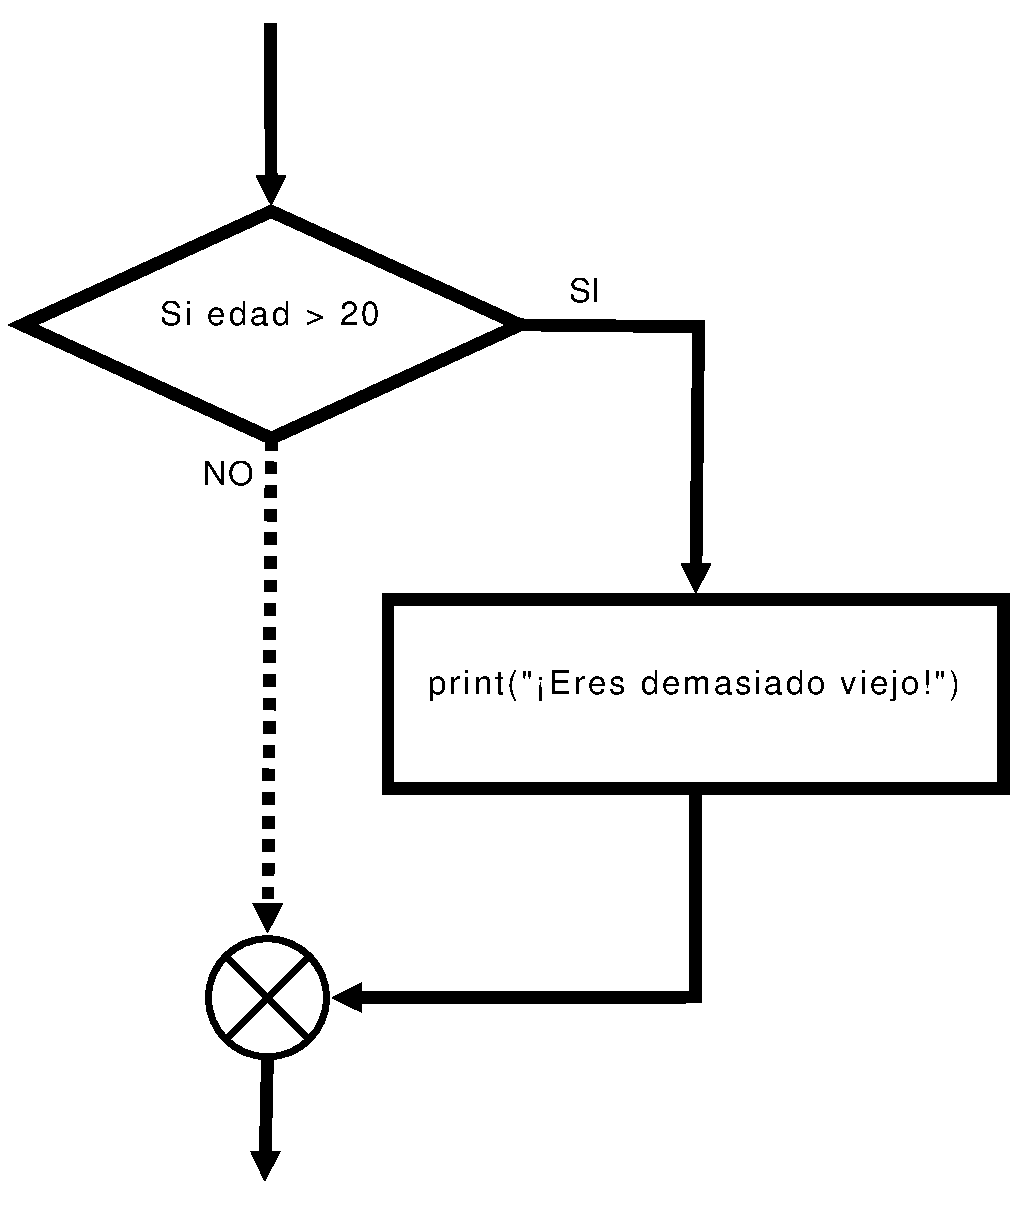
\includegraphics[width=72mm]{if1.eps}
\end{center}
\caption{Diagrama de ejecución de la sentencia if}\label{if1}
\end{figure}

\par
Una condición\index{condiciones} es un cálculo de programación cuyo resultado es `Sí' (True) o `No' (False).  Hay ciertos símbolos (u operadores) que se utilizan para crear condiciones, como son:

\begin{center}
\begin{tabular}{|c|c|}
\hline
== & igual \\
\hline
!= & no igual o distinto de \\
\hline
$>$ & mayor que \\
\hline
$<$ & menor que \\
\hline
$>$= & mayor o igual que \\
\hline
$<$= & menor o igual que \\
\hline
\end{tabular}
\end{center}

Por ejemplo, si tienes 10 años, entonces la condición \code{tu\_edad == 10} tendría como resultado True (Sí), pero si no tienes 10 años, devolvería False (No).  Recuerda: no confundas los \textbf{dos} símbolos de igual (==) utilizados para las condiciones, con el símbolo de igual utilizado para asignar valores (=)---si utilizas un único símbolo = en una \emph{condición}, Python devolverá un mensaje de error.
\par
Si asumimos que asignas tu edad a la variable \code{edad}, entonces si tienes 12 años, la condición$\ldots$

\begin{listing}
\begin{verbatim}
edad > 10
\end{verbatim}
\end{listing}

$\ldots$ daría como resultado el valor True.  Si tuvieras 8 años, el resultado sería False.  Si tuvieras 10 años, el resultado también seguiría siendo False---porque la condición comprueba que sea mayor que ($>$) 10, y no mayor o igual ($>$=) que 10.

Vamos a probar varios ejemplos:

\begin{listing}
\begin{verbatim}
>>> edad = 10
>>> if edad > 10:
...     print('llegué aquí')
\end{verbatim}
\end{listing}

\noindent
Si teclearas el ejemplo anterior en la consola, ¿Qué sucedería?
\par
\noindent
Nada.
\par
\noindent
El valor de la variable \code{edad} no es mayor que 10, por eso el bloque interior a la sentencia if (la sentencia print) no se ejecutará. Se puede observar lo que sudece en la figura~\ref{if2}

\begin{figure}
\begin{center}
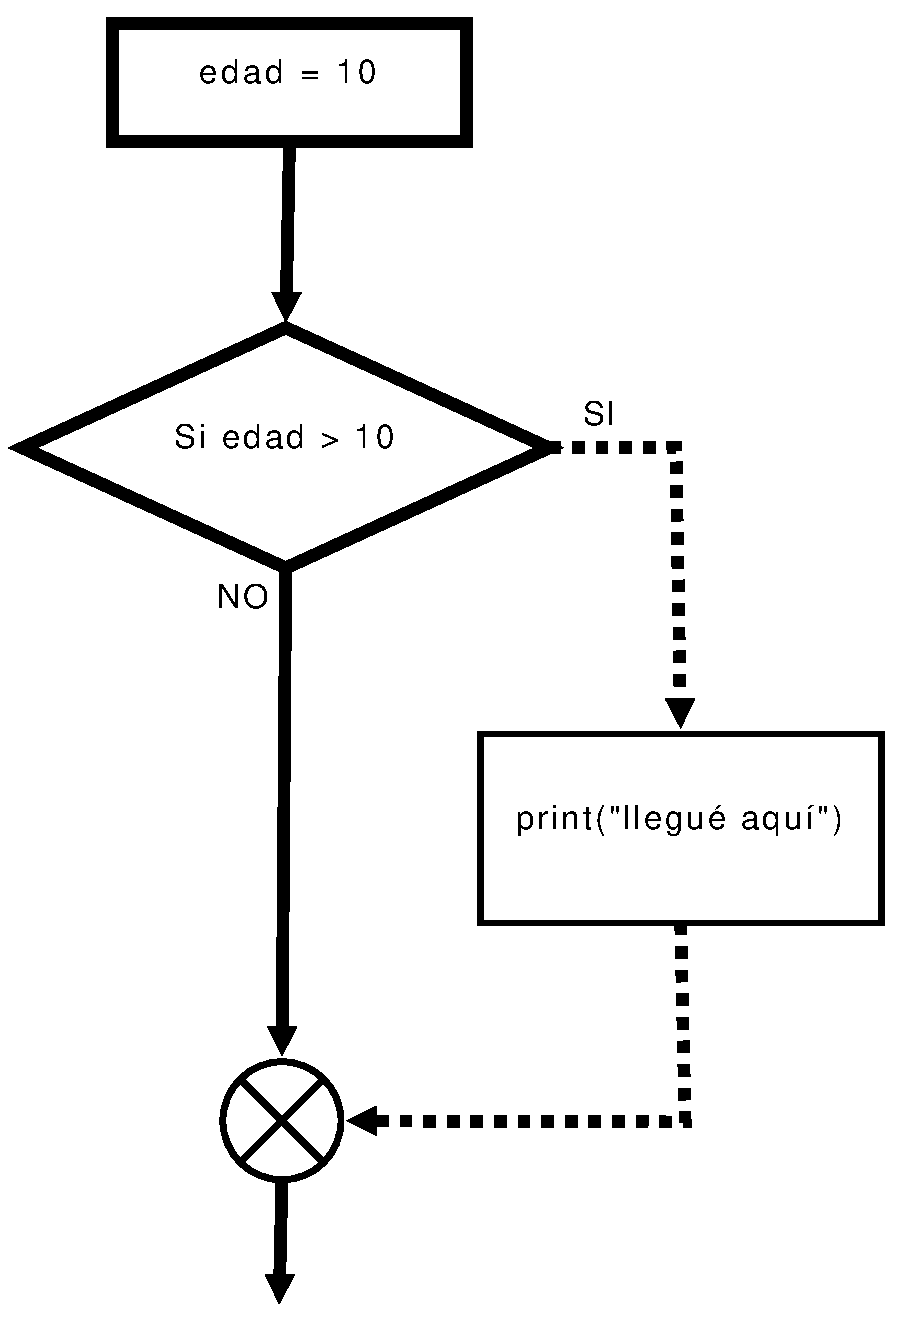
\includegraphics[width=72mm]{if2.eps}
\end{center}
\caption{Otro flujo de ejecución de una sentencia if.}\label{if2}
\end{figure}

Y qué pasará con el siguiente ejemplo:

\begin{listing}
\begin{verbatim}
>>> edad = 10
>>> if edad >= 10:
...     print('llegué aquí')
\end{verbatim}
\end{listing}

Si pruebas este ejemplo en la consola, entonces deberías ver el mensaje `llegué aquí' impreso en la consola. La figura~\ref{if3} muestra la ejecución.

\begin{figure}
\begin{center}
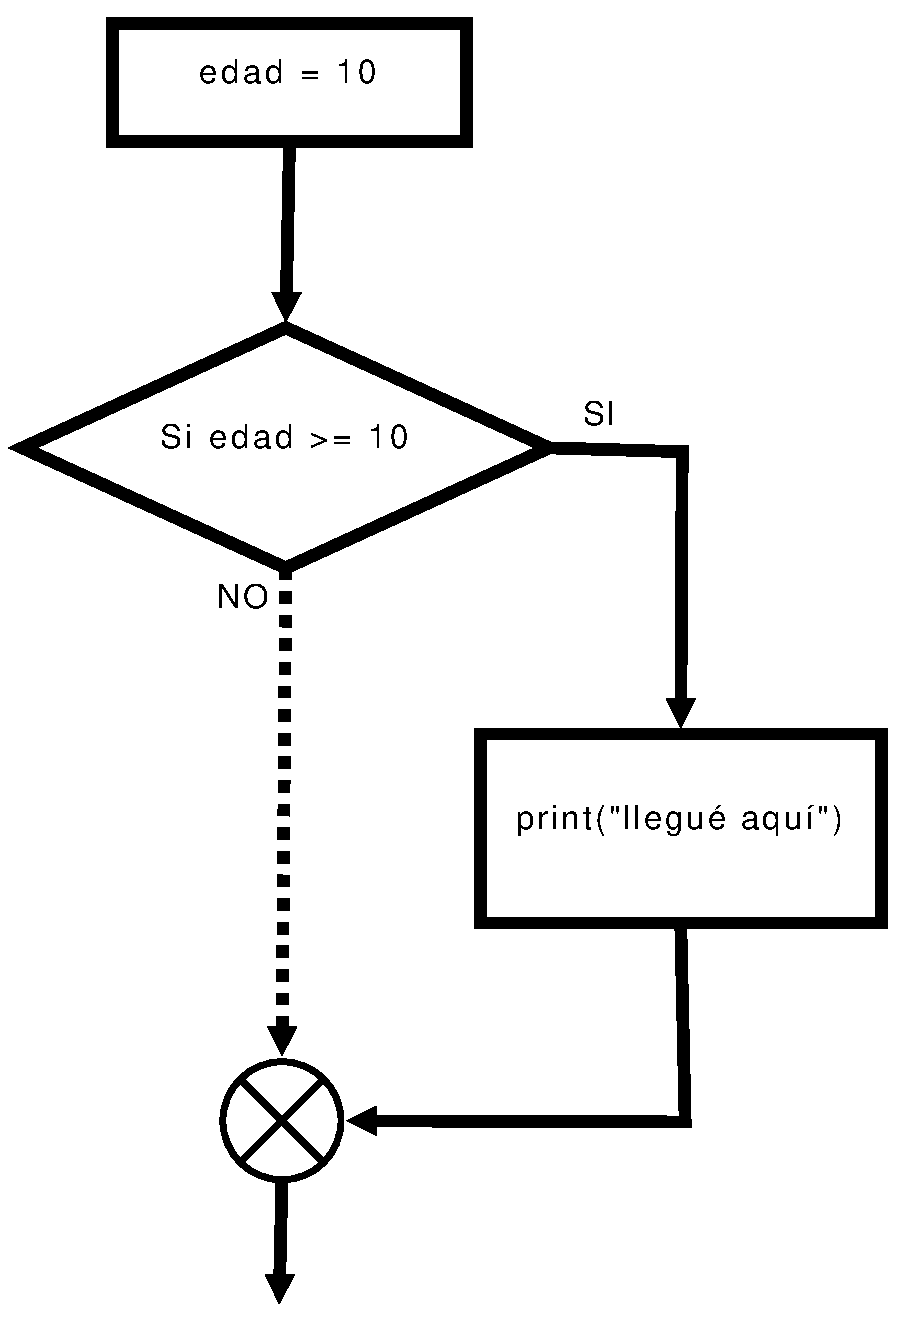
\includegraphics[width=72mm]{if3.eps}
\end{center}
\caption{Otro flujo de ejecución del ejemplo anterior.}\label{if3}
\end{figure}

Lo mismo sucederá con el siguiente ejemplo:

\begin{listing}
\begin{verbatim}
>>> edad = 10
>>> if edad == 10:
...     print('llegué aquí')
llegué aquí
\end{verbatim}
\end{listing}

Que se muestra en la figura~\ref{if4}.

\begin{figure}
\begin{center}
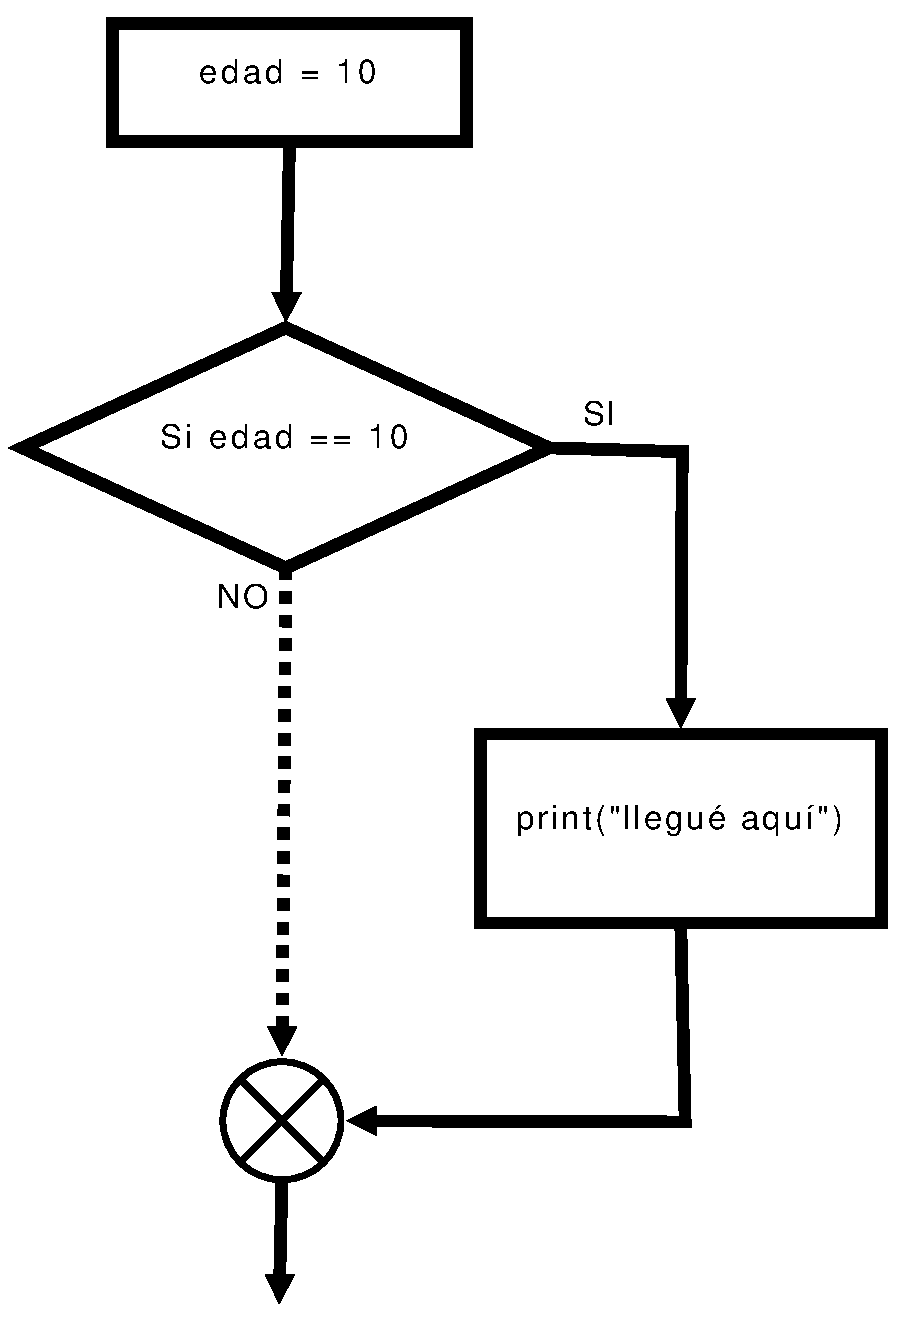
\includegraphics[width=72mm]{if4.eps}
\end{center}
\caption{Otro flujo más.}\label{if4}
\end{figure}

\section{Haz esto$\ldots$ o ¡¡¡SI NO!!!}

Podemos extender una sentencia if, para que haga algo cuando una condición no sea verdadera.  Por ejemplo, imprimir la palabra `Hola' en la consola si tu edad es de 12 años, pero imprimir `Adiós' si no lo es.  Para hacer esto, utilizamos una sentencia if-then-else\index{if then else - sentencia} (es una forma de decir \emph{``si algo es verdad, entonces haz \textbf{esto}, en caso contrario haz \textbf{esto otro}''}):

\begin{listing}
\begin{verbatim}
>>> edad = 12
>>> if edad == 12:
...     print('Hola')
... else:
...     print('Adiós')
Hola
\end{verbatim}
\end{listing}


Teclea el ejemplo anterior y verás la palabra `Hola' en la consola. El diagrama de ejecución de este ejemplo es como se muestra en la figura~\ref{if5}. 

\begin{figure}
\begin{center}
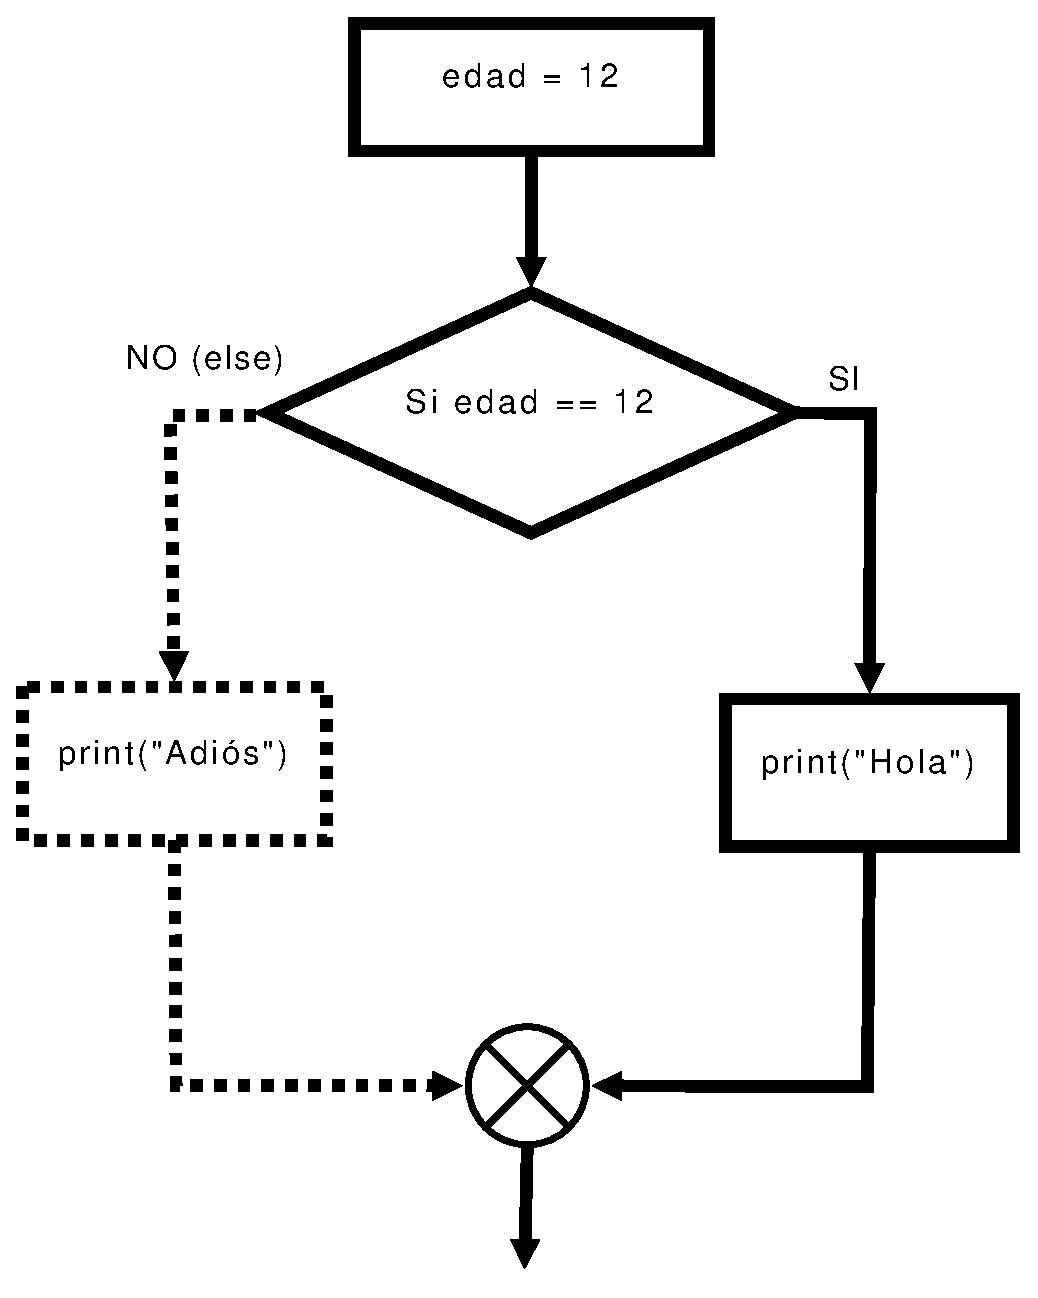
\includegraphics[width=90mm]{if5.eps}
\end{center}
\caption{Flujo de ejecución de una setencia if-else.}\label{if5}
\end{figure}

Cambia el valor de la variable \code{edad} a otro número y verás que se imprime la palabra `Adiós':

\begin{listing}
\begin{verbatim}
>>> edad = 8
>>> if edad == 12:
...     print('Hola')
... else:
...     print('Adiós')

Adiós
\end{verbatim}
\end{listing}

Ahora la edad no es 12 por lo que la ejecución varía. El digrama de la figura~\ref{if6} muestra que la ejecución ahora es diferente al de la figura~\ref{if5}.

\begin{figure}
\begin{center}
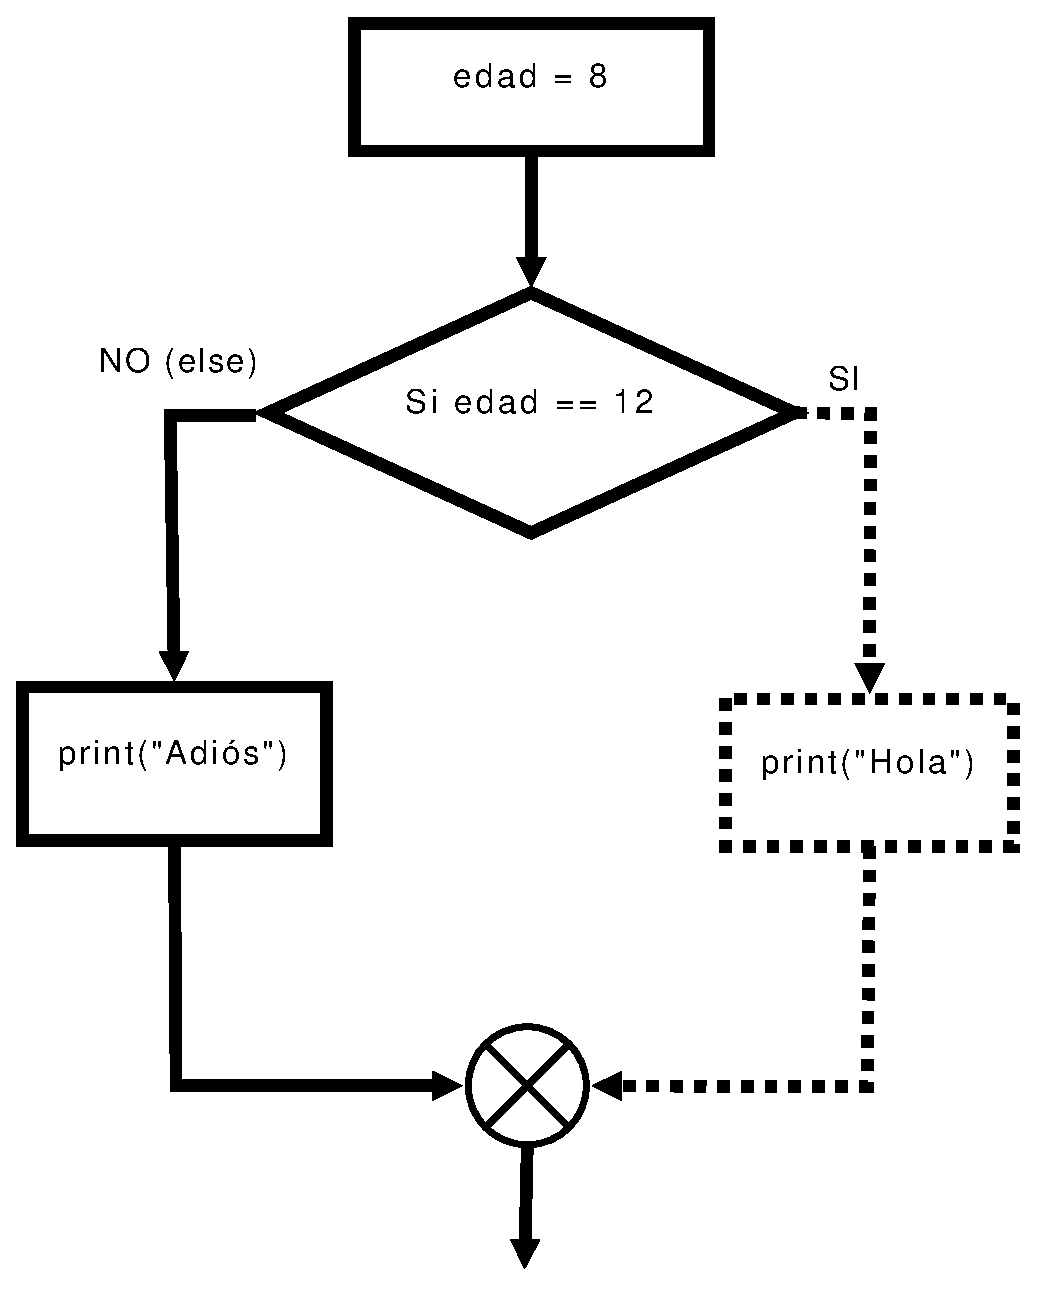
\includegraphics[width=90mm]{if6.eps}
\end{center}
\caption{Flujo de ejecución que sigue el camino del else.}\label{if6}
\end{figure}

\section{Haz esto$\ldots$ o haz esto$\ldots$ o haz esto$\ldots$ o ¡¡¡SI NO!!!}

Podemos extender aún más la sentencia if utilizando elif (contracción de else-if).  Por ejemplo, podemos preguntar si tu edad es 10, o si es 11, o si es 12 y así cuanto queramos: 

\begin{listing}
\begin{verbatim}
 1. >>> edad = 12
 2. >>> if edad == 10:
 3. ...     print('tienes 10 años')
 4. ... elif edad == 11:
 5. ...     print('tienes 11 años')
 6. ... elif edad == 12:
 7. ...     print('tienes 12 años')
 8. ... elif edad == 13:
 9. ...     print('tienes 13 años')
10. ... else:
11. ...     print('¿Eh?')
12. ...
13. tienes 12 años
\end{verbatim}
\end{listing}

En el código anterior, la línea 2 pregunta si el valor de la variable edad es igual a 10.  Si no lo es, entonces salta a la línea 4 sin ejecutar la 3. En la línea 4 valida si el valor de la variable edad es igual a 11. De nuevo no lo es, por eso salta a la línea 6 sin ejecutar la 5.  Este caso, comprueba el valor y sí que es igual a 12.  Por eso Python ejecuta el bloque de la línea 7, y ejecuta esa sentencia print.  (Espero que te hayas dado cuenta de que hay 5 grupos en este código---líneas 3, 5, 7, 9 y 11).  Después, una vez ejecutado un bloque, no se pregunta por ninguna de las condiciones que están después y se salta al final de todos los if, después del else en la línea 12.

¿Complicado? Un poco. Observa la figura~\ref{if7} para tratar de entenderlo un poco mejor.

\begin{figure}
\begin{center}
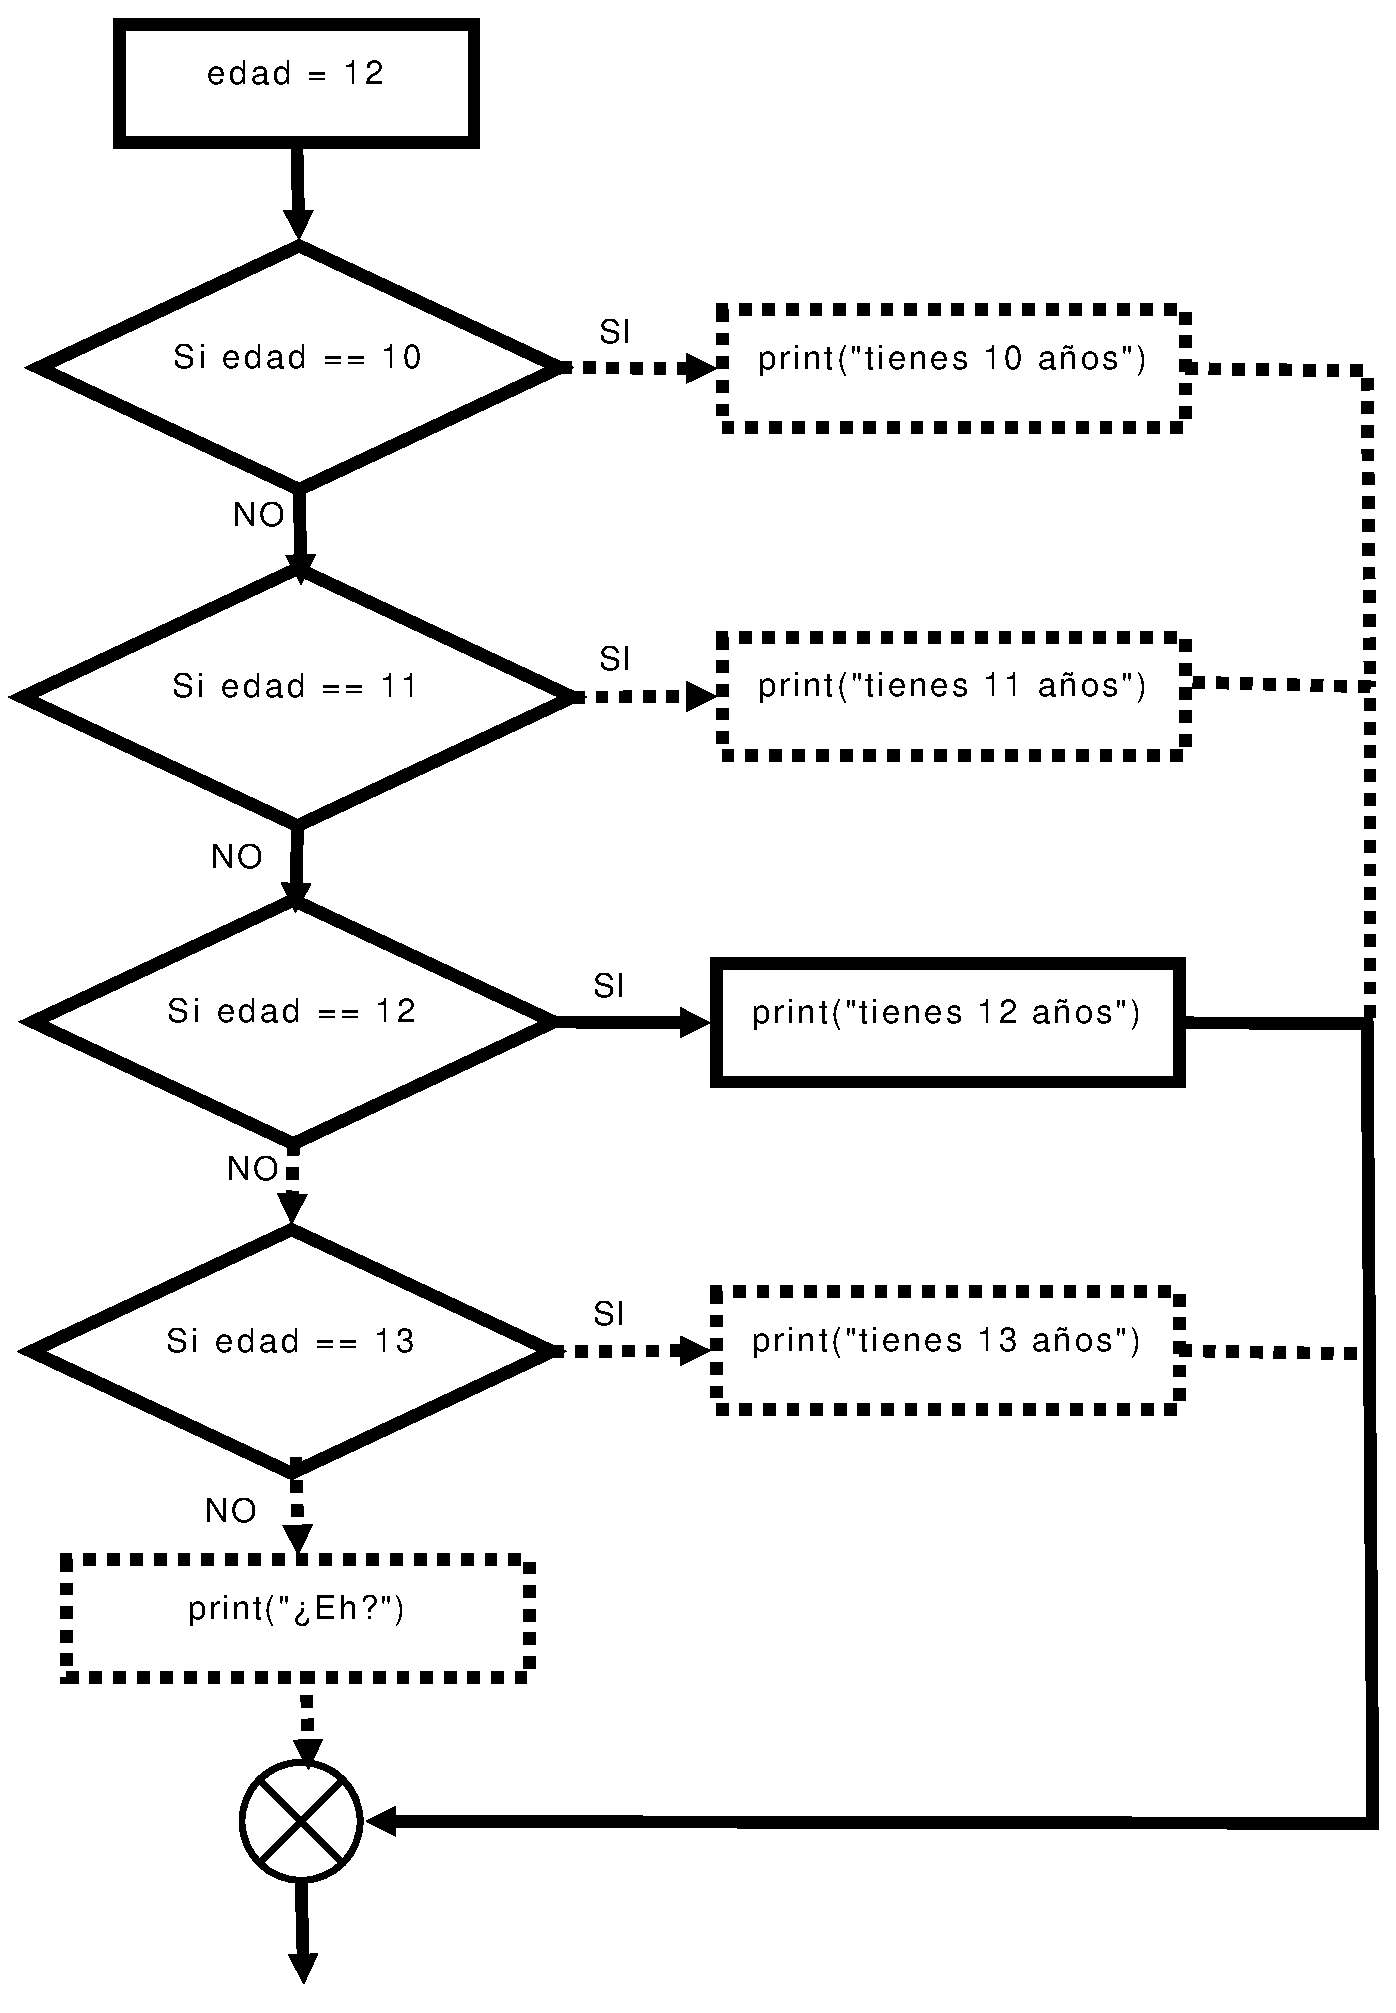
\includegraphics[width=90mm]{if7.eps}
\end{center}
\caption{Múltiples caminos posibles gracias al uso de elif.}\label{if7}
\end{figure}

\section{Combinando condiciones}\index{condiciones!combinando}
Puedes combinar condiciones utilizando las palabras `and' y `or'\footnote{En inglés significan `Y' y `O'}. Así podemos comprimir el ejemplo anterior un poco, utilizando `or' para unir condiciones:

\begin{listing}
\begin{verbatim}
1. >>> if edad == 10 or edad == 11 or edad == 12 or edad == 13:
2. ...     print('tienes %s años' % edad)
3. ... else:
4. ...     print('¿Eh?')
\end{verbatim}
\end{listing}

Si alguna de las condiciones de la línea 1 es verdadera (por ejemplo, si la variable edad vale 10 \textbf{o} vale 11 \textbf{o} vale 12 \textbf{o} vale 13), entonces se ejecuta el bloque de código de la línea 2, en otro caso Python continúa en la línea 4.  

El diagrama de la figura~\ref{if8} muestra que el or es parecido al elif en la forma en la que se comprueba cada parte de la condición. Basta con que una de ellas sea cierta para que se ejecute el bloque que contiene el if. En caso de no ser ninguna cierta se ejecuta el bloque de sentencias del else.

\begin{figure}
\begin{center}
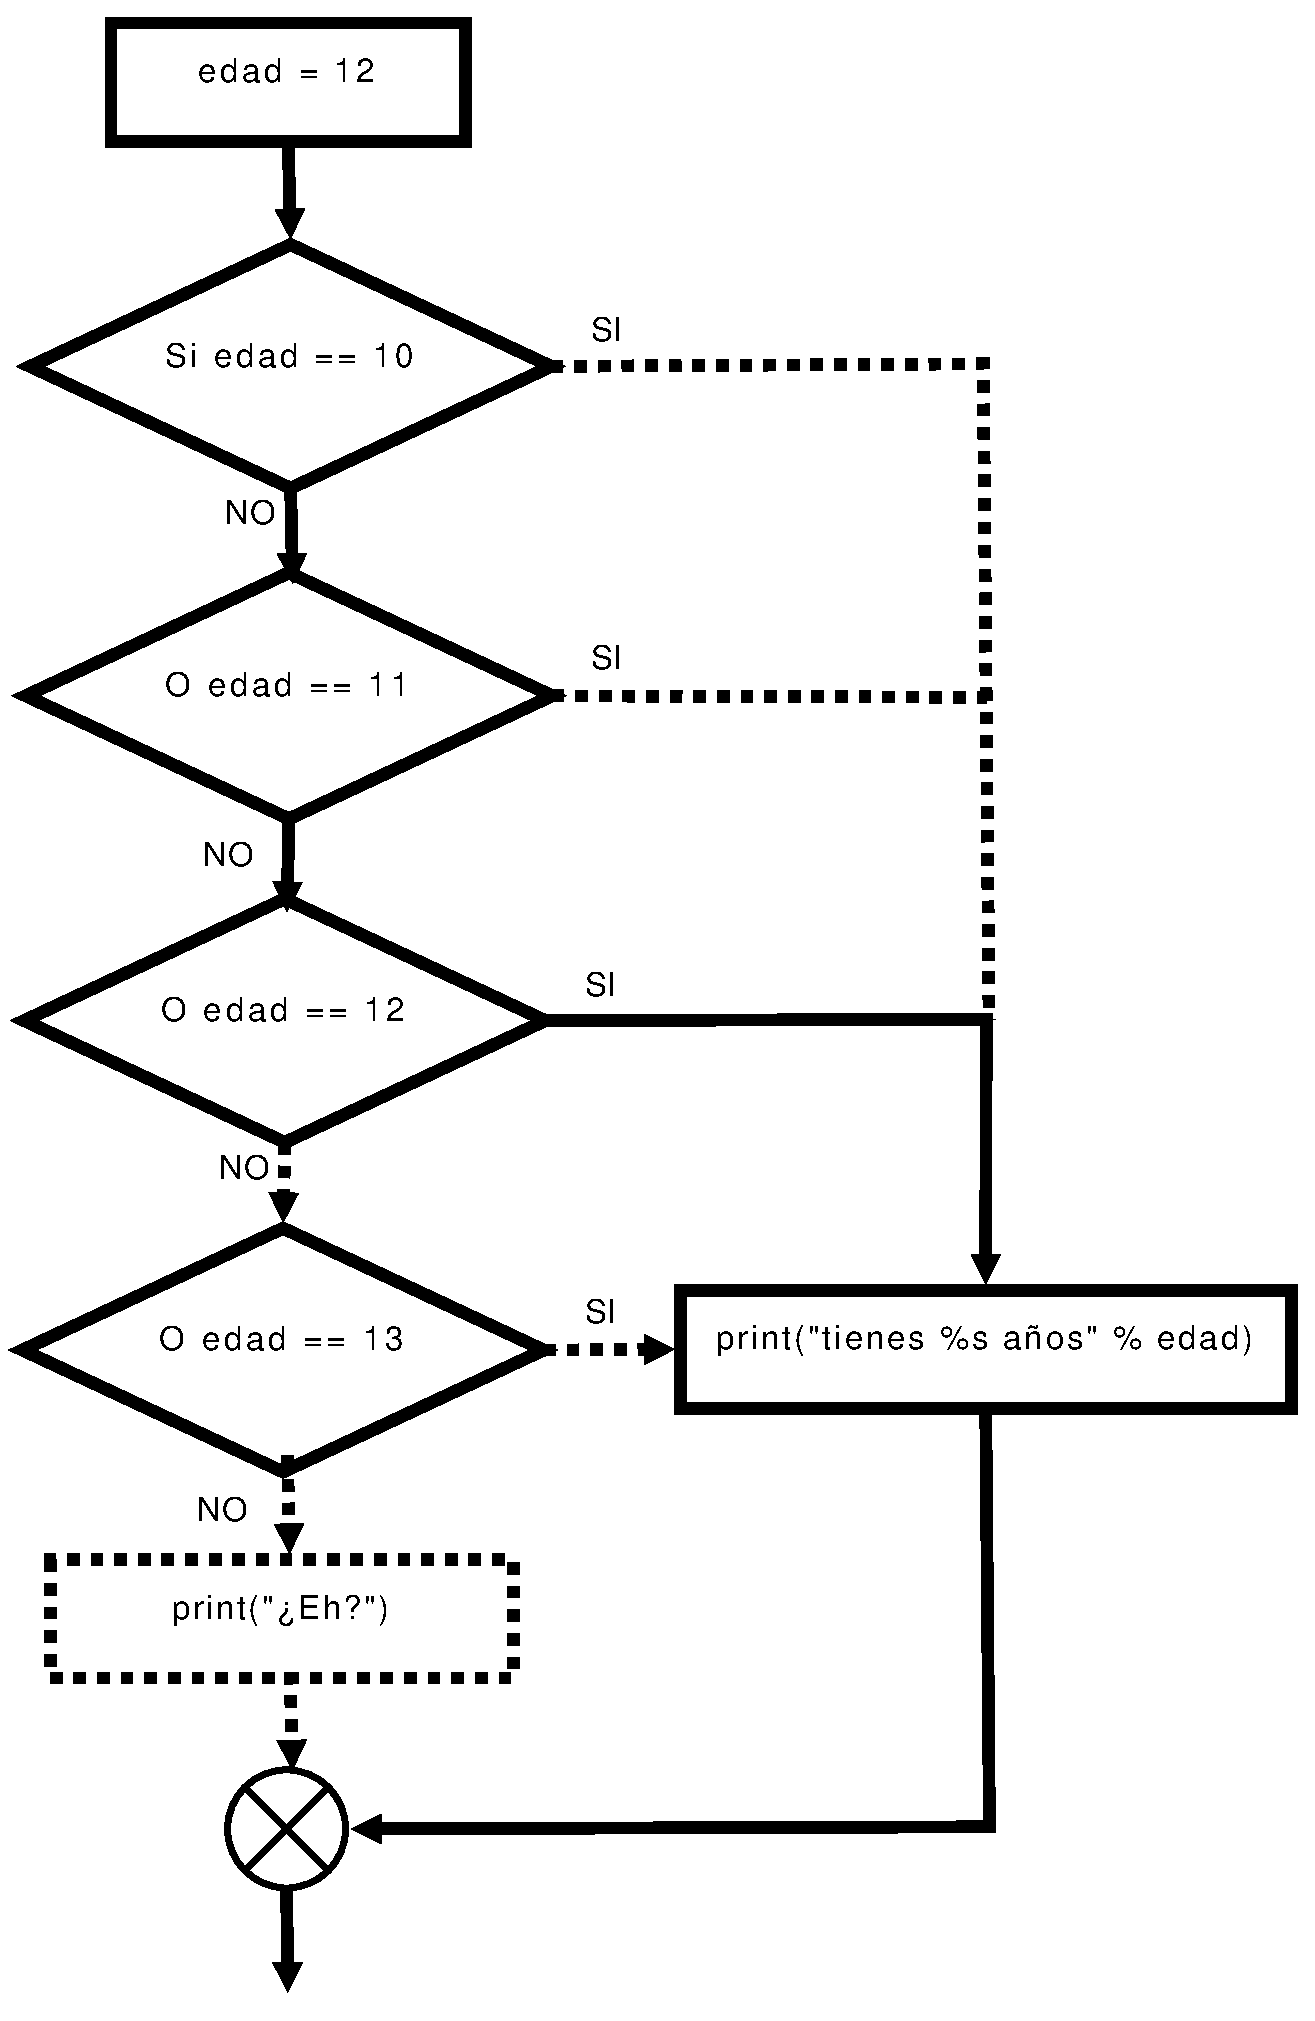
\includegraphics[width=90mm]{if8.eps}
\end{center}
\caption{Condiciones complejas usando \emph{or}.}\label{if8}
\end{figure}

Aún podemos mejorar un poquito más el ejemplo mediante el uso de la palabra `and' y los símbolos $>$= y $<$=.

\begin{listing}
\begin{verbatim}
1. >>> if edad >= 10 and edad <= 13:
2. ...     print('tienes %s años' % edad)
3. ... else:
4. ...     print('¿Eh?')
\end{verbatim}
\end{listing}

Seguramente te has figurado ya que si son verdaderas (True) \textbf{ambas} condiciones de la línea 1 entonces se ejecuta el bloque de código de la línea 2 (si la edad es mayor o igual que 10 \textbf{y} menor o igual que 13). Así que si la variable edad vale 12, se mostrará en la consola la frase `tienes 12 años': puesto que 12 es mayor o igual que 10 y menor o igual que 13.  

El diagrama de la figura~\ref{if9} muestra que el uso del and hace que sea necesario cumplir todas las condiciones incluidas para que se pueda ejecutar el bloque de sentencias del if. En cuanto haya una condición que no se cumpla se ejecuta en su lugar el bloque de sentencias correspondiente al else.

\begin{figure}
\begin{center}
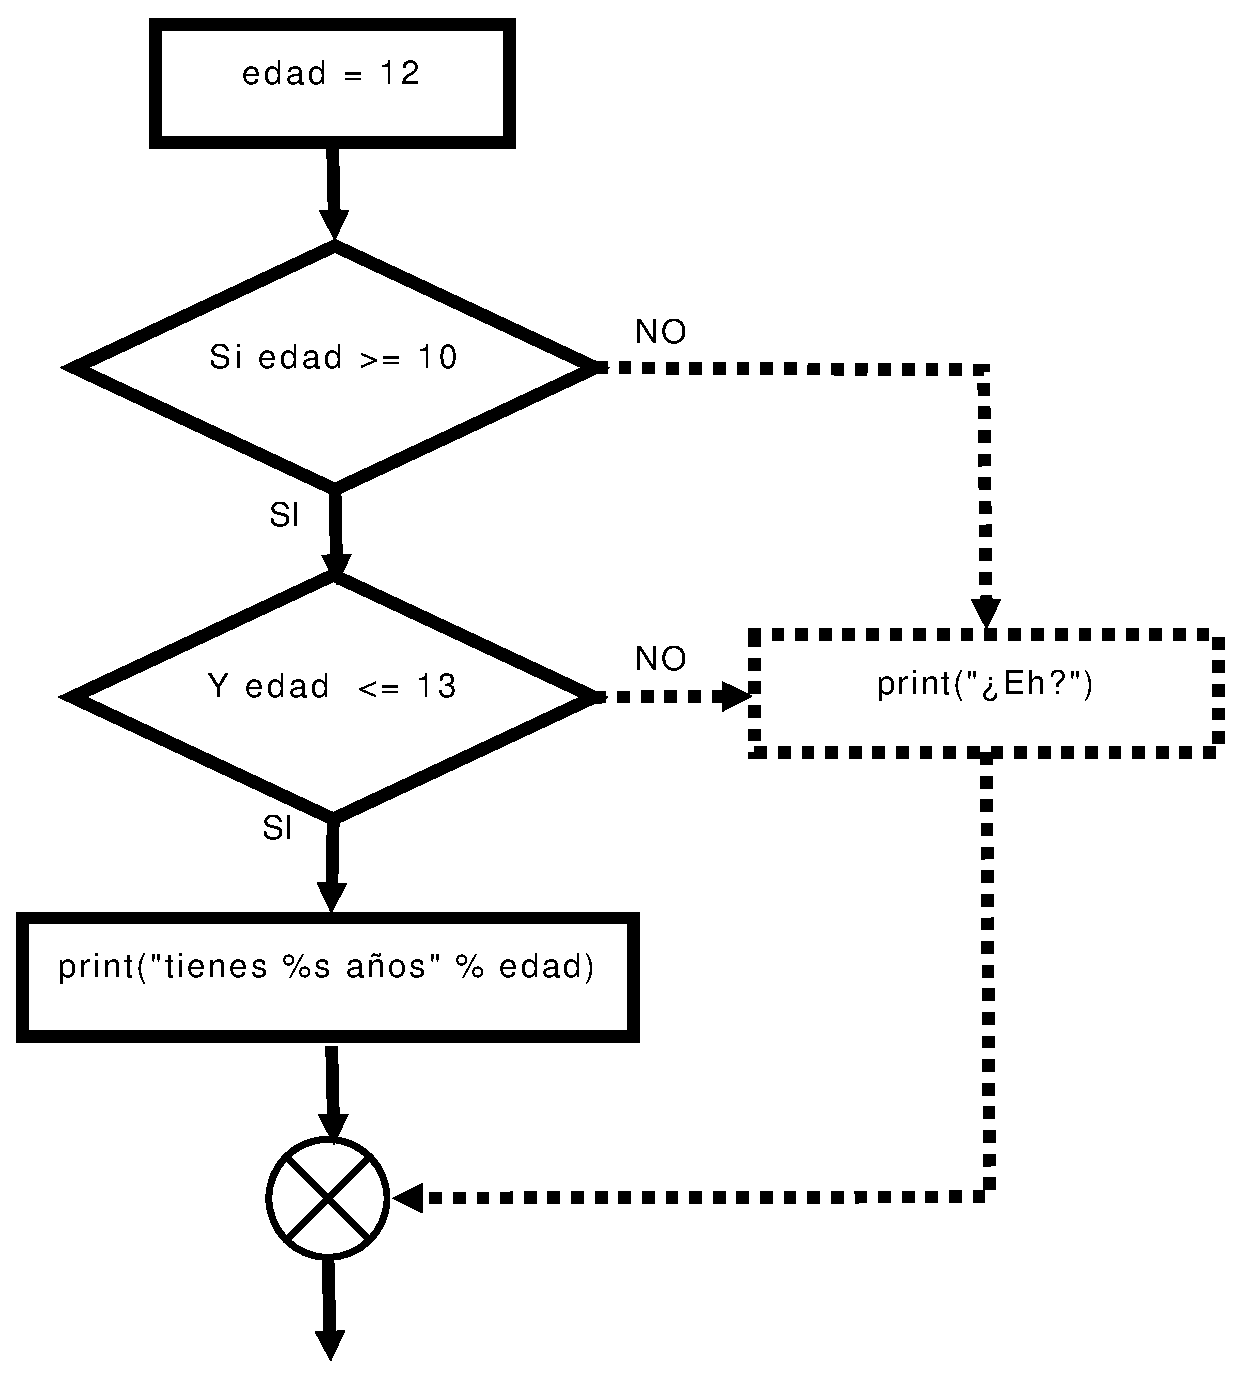
\includegraphics[width=90mm]{if9.eps}
\end{center}
\caption{Condiciones complejas usando \emph{and}.}\label{if9}
\end{figure}

\section{Vacío}\index{None}

Hay otra clase de valor que se puede asignar a una variable del que no hablamos en el capítulo anterior:  \textbf{Nada}.
\par
De igual forma que podemos asignar a una variable valores que representan números, cadenas y listas, 'nada' también es un valor que se puede asignar.  En Python, el valor que representa el vacío, la nada, se escribe como \code{None}\footnote{En inglés `None' significa `Ninguno'} (En otros lenguajes de programación se llama Null) y se puede utilizar del mismo modo que otros valores:

\begin{listing}
\begin{verbatim}
>>> mivalor = None
>>> print(mivalor)
None
\end{verbatim}
\end{listing}

None se suele utilizar para quitarle el valor que tenía una variable, de forma que esté `limpia'. También se suele utilizar para crear una variable sin asignarle un valor antes de que se utilice.
\par
Por ejemplo, si todos los miembros de tu equipo de fútbol estuviérais consiguiendo fondos para comprar unos uniformes nuevos, y te tocase contar cuanto dinero se ha recoletado, Posiblemente quisieras esperar hasta que todo el equipo hubiera regresado con el dinero que ha conseguido cada uno antes de comenzar a sumarlo todo.  En términos de programación, podríamos crear una variable para cada miembro del equipo, asignándole a cada una de ellas el valor None:

\begin{listing}
\begin{verbatim}
>>> jugador1 = None
>>> jugador2 = None
>>> jugador3 = None
\end{verbatim}
\end{listing}

Entonces podríamos utilizar la sentencia if para validar si todos los miembros del equipo han vuelto con el dinero:

\begin{listing}
\begin{verbatim}
>>> if jugador1 is None or jugador2 is None or jugador3 is None:
...     print('Por favor, espera a que vuelvan todos los jugadores')
... else:
...     print('Has conseguido %s euros' % (jugador1 + jugador2 + jugador3))
\end{verbatim}
\end{listing}

La sentencia if del ejemplo valida si alguna de las variables tiene el valor \code{None}, e imprime el primer mensaje si es así.  Si todas las variables tienen un valor real (algún número) se imprime el segundo mensaje que suma el dinero total antes de hacerlo.   Si pruebas el código anterior con todas las variables valiendo None, verás el primer mensaje en la consola (no te olvides de crear primero las variables o Python mostrará un mensaje de error): 

\begin{listing}
\begin{verbatim}
>>> if jugador1 is None or jugador2 is None or jugador3 is None:
...     print('Por favor, espera a que vuelvan todos los jugadores')
... else:
...     print('Has conseguido %s euros' % (jugador1 + jugador2 + jugador3))
Por favor, espera a que vuelvan todos los jugadores
\end{verbatim}
\end{listing}

Si asignamos algún valor a una o a dos variables aún se imprime el mismo mensaje:

\begin{listing}
\begin{verbatim}
>>> jugador1 = 100
>>> jugador3 = 300
>>> if jugador1 is None or jugador2 is None or jugador3 is None:
...     print('Por favor, espera a que vuelvan todos los jugadores')
... else:
...     print('Has conseguido %s euros' % (jugador1 + jugador2 + jugador3))
Por favor, espera a que vuelvan todos los jugadores
\end{verbatim}
\end{listing}

\noindent
Finalmente, cuando asignamos valor a todas las variables el resultado es la suma de todos los valores y, por lo tanto, el dinero que hemos recolectado:

\begin{listing}
\begin{verbatim}
>>> jugador1 = 100
>>> jugador3 = 300
>>> jugador2 = 500
>>> if jugador1 is None or jugador2 is None or jugador3 is None:
...     print('Por favor, espera a que vuelvan todos los jugadores')
... else:
...     print('Has conseguido %s euros' % (jugador1 + jugador2 + jugador3))
Has conseguido 900 euros
\end{verbatim}
\end{listing}

\section{¿Cuál es la diferencia$\ldots$?}\label{whatsthedifference}\index{igualdad}

¿Cuál es la diferencia entre \code{10} y \code{'10'}?
\par
Podrías decir que no mucha aparte de las comillas.  Bien, de la lectura de los capítulos anteriores, sabes que el primero es un número y que el segundo es una cadena. Esto los hace ser más distintos de lo que podrías imaginar.  Antes comparamos el valor de una variable (edad) con un número en una sentencia if:

\begin{listing}
\begin{verbatim}
>>> if edad == 10:
...     print('tienes 10 años')
\end{verbatim}
\end{listing}

Si asignas el valor 10 a la variable edad, se imprimirá la cadena en la consola:

\begin{listing}
\begin{verbatim}
>>> edad = 10
>>> if edad == 10:
...     print('tienes 10 años')
...
tienes 10 años
\end{verbatim}
\end{listing}

Si embargo si lo que asignas a la variable edad es el valor \code{'10'} (observa las comillas), entonces no se imprimirá la cadena:

\begin{listing}
\begin{verbatim}
>>> edad = '10'
>>> if edad == 10:
...     print('tienes 10 años')
...
\end{verbatim}
\end{listing}

¿Porqué no se ejecuta el código del bloque interior al if?  Porque una cadena siempre es diferente a un número, incluso aunque se parezcan:

\begin{listing}
\begin{verbatim}
>>> edad1 = 10
>>> edad2 = '10'
>>> print(edad1)
10
>>> print(edad2)
10
\end{verbatim}
\end{listing}

¡Ves!  Parecen exactamente lo mismo.  Pero, como uno es una cadena y el otro es un número, son valores diferentes.  Por eso edad == 10 (edad igual a 10) nunca será True (verdadero) cuando la variable edad contiene un valor que es una cadena.
\par
Posiblemente la mejor manera de imaginártelo es considerar 10 libros y 10 ladrillos.  El número de elementos puede que sea el mismo, no puedes decir que 10 libros sean igual que 10 ladrillos, ¿o sí?  Afortunadamente en Python existen funciones mágicas que puede convertir cadenas en números y números en cadenas (aunque nunca convertirán ladrillos en libros). Por ejemplo, para convertir la cadena `10' en un número puedes utilizar la función \code{int}\footnote{`int' es la contracción de `integer' que significa `entero' en inglés y se refiere a los números enteros: 0, 1, 2,... y también -1, -2, -3, ...}:

\begin{listing}
\begin{verbatim}
>>> edad = '10'
>>> edad_convertida = int(edad)
\end{verbatim}
\end{listing}

\noindent
La variable edad\_convertida contiene el \textbf{número} 10, y no una cadena. Para convertir un número en una cadena, podrías utilizar la función \code{str}\footnote{`str' es la contracción de `string' que significa `cadena' en inglés}:

\begin{listing}
\begin{verbatim}
>>> edad = 10
>>> edad_convertida = str(edad)
\end{verbatim}
\end{listing}

\noindent
La variable edad\_convertida contiene ahora la \textbf{cadena} `10', y no un número.  Si volvemos ahora a la sentencia if que no imprimía nada:

\begin{listing}
\begin{verbatim}
>>> edad = '10'
>>> if edad == 10:
...     print('tienes 10 años')
...
\end{verbatim}
\end{listing}

\noindent
Si convirtiéramos la variable \emph{antes} de la validación, entonces el resultado sería diferente:

\begin{listing}
\begin{verbatim}
>>> edad = '10'
>>> edad_convertida = int(edad)
>>> if edad_convertida == 10:
...     print('tienes 10 años')
...
tienes 10 años
\end{verbatim}
\end{listing}

\section{Cosas que puedes probar}

\emph{En este capitulo hemos visto que la sentencia if nos permite preguntar por valores de una variable y decidir qué código queremos ejecutar según el resultado sea Verdadero (True) o Falso (False)}.

\subsection*{Ejercicio 1}
¿Qué crees que se imprimirá en pantalla al ejecutar este código?

\begin{listing}
\begin{verbatim}
>>> valor = 1000
>>> if valor > 100:
...     print('Tengo una moto')
... else:
...     print('Tengo un coche')
\end{verbatim}
\end{listing}

¿Y al ejecutar este otro?

\begin{listing}
\begin{verbatim}
>>> valor1 = 30
>>> valor2 = 80
>>> if valor1 + valor2 < 100:
...     print('Tengo una moto')
... else:
...     print('Tengo un coche')
\end{verbatim}
\end{listing}

\subsection*{Ejercicio 2}
Crea una variable con el valor que quieras. Luego utiliza una sentencia if para que se imprima en consola la palabra 'hola' si la variable tiene un valor menor que 100, la palabra 'chao' si la variable vale entre 100 y 200, y la palabra 'adiós' si el valor de la variable es cualquier otro (Pista: recuerda que puedes usar la opción else y la palabra and para poner dos condiciones en un mismo if).

\newpage
